\newpage
\section{On-Device AI Module: Predictive TinyML Pipeline}
\label{sec:tinyml}

This section specifies the deployed TinyML path used by H.E.R.A for
on-device anomaly scoring on ESP32-S3. The pipeline is fixed as a
next-value prediction problem with a TFLite-deployable MLP runtime.

\subsection{Problem Formulation}
\label{sec:tinyml-formulation}

At time index $t$, let sensor vector
$\mathbf{r}_t = [T_t, H_t]^\top \in \mathbb{R}^2$ contain temperature
and humidity.

A window of size $N=10$ is used:
\begin{equation}
\label{eq:window-input}
\mathbf{X}_t = [\mathbf{r}_{t-N}, \mathbf{r}_{t-N+1}, \dots, \mathbf{r}_{t-1}] 
\in \mathbb{R}^{10 \times 2}.
\end{equation}

Model output is the one-step forecast:
\begin{equation}
\label{eq:next-prediction}
\hat{\mathbf{r}}_t = f_\theta(\mathbf{X}_t).
\end{equation}

Prediction residual:
\begin{equation}
\label{eq:residual}
\mathbf{e}_t = \hat{\mathbf{r}}_t - \mathbf{r}_t.
\end{equation}

Operational anomaly score:
\begin{equation}
\label{eq:anomaly-score}
    s_t = \frac{\lVert \mathbf{e}_t \rVert_2}{\sigma_{\text{train}}}.
\end{equation}

Decision rule:
\begin{equation}
\label{eq:anomaly-rule}
\text{anomaly}_t =
\begin{cases}
1, & s_t > \tau_a \\
0, & s_t \leq \tau_a
\end{cases}
\quad \text{with} \quad \tau_a = 1.0.
\end{equation}

\subsection{Data Representation and Preprocessing}
\label{sec:tinyml-data}

Training source is \texttt{HCMC\_temp\_humid\_raw.csv} with three
columns: temperature, humidity, and binary label.

\begin{table}[H]
\centering
\caption{Dataset statistics used in the final TinyML pipeline.}
\label{tab:data-stats}
\renewcommand{\arraystretch}{1.25}
\begin{tabular}{l c}
    \toprule
    \textbf{Property} & \textbf{Value} \\
    \midrule
    Total records              & 1,000 \\
    Normal records (label=0)   & 805 \\
    Anomaly records (label=1)  & 195 \\
    Window size $N$            & 10 \\
    Generated sequences        & 795 \\
    Train/test split           & 80\% / 20\% \\
    Random seed                & 42 \\
    \bottomrule
\end{tabular}
\end{table}

Only label $=0$ samples are used for model fitting.

Feature normalization is standard score per channel:
\begin{equation}
\label{eq:zscore}
\tilde{x}_i = \frac{x_i - \mu_i}{\sigma_i + \epsilon}, \quad \epsilon=10^{-7}.
\end{equation}

The exported statistics file
\texttt{dht\_predictive\_model\_stats.csv} stores
$\mu_T, \sigma_T, \mu_H, \sigma_H$ for identical inference-time scaling
on ESP32.

\subsection{Model Set and Selection Logic}
\label{sec:tinyml-models}

The training pipeline evaluates six regressors on the same split:
\begin{enumerate}
    \item Dense MLP (Keras, TFLite-compatible)
    \item Random Forest Regressor
    \item Gradient Boosting Regressor
    \item SVR (RBF kernel)
    \item KNN Regressor
    \item Ridge Regression
\end{enumerate}

Selection constraints are:
\begin{itemize}
    \item primary metric: minimum MSE,
    \item deployability constraint: model must run on TFLite Micro,
    \item memory constraint: fit microcontroller flash/RAM envelope.
\end{itemize}

Therefore, final deployment is chosen by:
\begin{equation}
\label{eq:deploy-choice}
\theta^* = \arg\min_{\theta \in \mathcal{D}} \text{MSE}(\theta),
\end{equation}
where $\mathcal{D}$ is the subset of deployable models.
In this project, $\mathcal{D}$ contains only the Dense MLP.

\subsection{Dense MLP Architecture}
\label{sec:tinyml-mlp}

\begin{table}[H]
\centering
\caption{Final deployable MLP architecture.}
\label{tab:model-dense}
\renewcommand{\arraystretch}{1.25}
\begin{tabular}{l c c c}
    \toprule
    \textbf{Layer} & \textbf{Output} & \textbf{Activation} & \textbf{Params} \\
    \midrule
    Flatten         & $(20,)$ & -      & 0   \\
    Dense           & $(20,)$ & ReLU   & 420 \\
    Dense           & $(16,)$ & ReLU   & 336 \\
    Dense           & $(8,)$  & ReLU   & 136 \\
    Dense (output)  & $(2,)$  & Linear & 18  \\
    \midrule
    \multicolumn{3}{l}{\textbf{Total}} & \textbf{910} \\
    \bottomrule
\end{tabular}
\end{table}

Training setup:
\begin{itemize}
    \item optimizer: Adam, learning rate $10^{-3}$,
    \item loss: MSE,
    \item batch size: 32,
    \item max epochs: 300,
    \item early stopping patience: 30,
    \item LR reduction patience: 15.
\end{itemize}

\subsection{Comparative Results}
\label{sec:tinyml-results}

\begin{table}[H]
\centering
\caption{Model comparison on held-out test split (sorted by MSE).}
\label{tab:comparison}
\renewcommand{\arraystretch}{1.25}
\begin{tabular}{l c c c c c}
    \toprule
    \textbf{Model} & \textbf{MSE}$\downarrow$ &
    \textbf{MAE}$\downarrow$ & \textbf{Size} &
    \textbf{Infer. (ms)} & \textbf{ESP32?} \\
    \midrule
    \textbf{Random Forest}  & \textbf{1.0062} & \textbf{0.8651}
                            & 2.6 MB  & 31.14 & No  \\
    Ridge                   & 1.0301 & 0.8739
                            & 609 B   & 0.046 & No  \\
    Dense (MLP)             & 1.0486 & 0.8853
                            & 5.9 KB  & $<0.01$ & \textbf{Yes} \\
    Gradient Boost          & 1.0804 & 0.8783
                            & 1.7 MB  & 0.493 & No  \\
    KNN                     & 1.0919 & 0.8820
                            & 56 KB   & 11.70 & No  \\
    SVR (RBF)               & 1.3488 & 0.9631
                            & 214 KB  & 0.296 & No  \\
    \bottomrule
\end{tabular}
\end{table}

Interpretation for deployment:
\begin{itemize}
    \item Random Forest is best in absolute MSE but not deployable to
          TFLite Micro runtime.
    \item Dense MLP is the best deployable candidate under embedded
          constraints.
    \item MLP binary size is 5,948 bytes, compatible with ESP32-S3
          firmware integration.
\end{itemize}

\subsection{Exported Artifacts and Build Outputs}
\label{sec:tinyml-artifacts}

After training, the pipeline keeps only deployment-relevant outputs in
\texttt{trained models/}:
\begin{enumerate}
    \item \texttt{dht\_predictive\_model.tflite}
    \item \texttt{dht\_predictive\_model.h}
    \item \texttt{dht\_predictive\_model\_stats.csv}
    \item \texttt{model\_comparison.csv}
\end{enumerate}

TFLite conversion:
\begin{lstlisting}[style=espCode, language=Python,
    caption={Final TFLite conversion path used in the training script.},
    label={lst:tflite-convert}]
converter = tf.lite.TFLiteConverter.from_keras_model(model)
converter.optimizations = [tf.lite.Optimize.DEFAULT]
converter.target_spec.supported_types = [tf.float16]
tflite_model = converter.convert()
\end{lstlisting}

C-header embedding format:
\begin{lstlisting}[style=espCode, language=C,
    caption={Generated C header layout for firmware embedding.},
    label={lst:c-header}]
const unsigned int dht_predictive_model_len = 5948;
alignas(8) const uint8_t dht_predictive_model[] = {
    0x20, 0x00, 0x00, 0x00, ...
};
\end{lstlisting}

\subsection{On-Device Inference Path}
\label{sec:tinyml-firmware}

Per sampling cycle:
\begin{enumerate}
    \item read $T_t, H_t$ from DHT20,
    \item normalize with exported $(\mu,\sigma)$,
    \item append into ring buffer of length $10 \times 2$,
    \item run TFLite Micro inference,
    \item compute $s_t$ using Equation~\ref{eq:anomaly-score},
    \item publish \texttt{inference\_result} via MQTT.
\end{enumerate}

\begin{figure}[H]
\centering
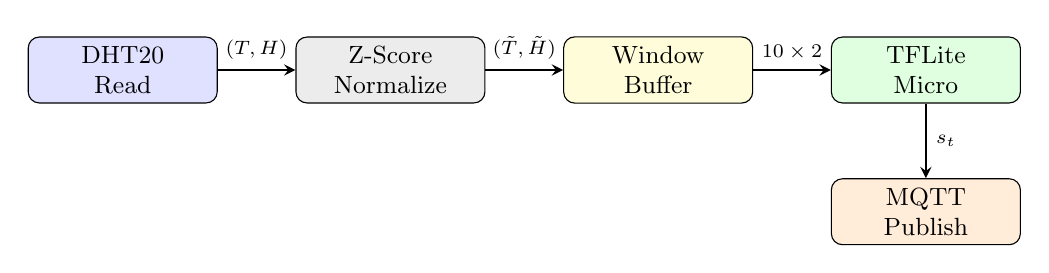
\begin{tikzpicture}[
    box/.style={draw, rounded corners, fill=#1, minimum width=2.4cm,
                minimum height=0.8cm, align=center, font=\small},
    arr/.style={->, >=stealth, thick},
]
\node[box=blue!12]   (dht)  at (0,0)    {DHT20\\Read};
\node[box=gray!15]   (norm) at (3.4,0)  {Z-Score\\Normalize};
\node[box=yellow!15] (buf)  at (6.8,0)  {Window\\Buffer};
\node[box=green!12]  (tfl)  at (10.2,0) {TFLite\\Micro};
\node[box=orange!15] (mqtt) at (10.2,-1.8) {MQTT\\Publish};

\draw[arr] (dht)  -- node[above,font=\scriptsize]{$(T,H)$} (norm);
\draw[arr] (norm) -- node[above,font=\scriptsize]{$(\tilde{T},\tilde{H})$} (buf);
\draw[arr] (buf)  -- node[above,font=\scriptsize]{$10 \times 2$} (tfl);
\draw[arr] (tfl)  -- node[right,font=\scriptsize]{$s_t$} (mqtt);
\end{tikzpicture}
\caption{Final on-device TinyML inference pipeline.}
\label{fig:inference-pipeline}
\end{figure}

\subsection{Interface to Multi-Agent Layer}
\label{sec:tinyml-to-mas}

Host-side MQTT service updates shared state with:
\begin{equation}
\label{eq:shared-state}
\texttt{sensor\_state} =
\{\texttt{temperature},\texttt{humidity},\texttt{inference\_result},
\texttt{led\_state},\texttt{neo\_led\_state},\texttt{last\_updated}\}.
\end{equation}

This state is consumed directly by:
\begin{itemize}
    \item Sensor Agent for status interpretation,
    \item Anomaly Agent for severity classification and explanation.
\end{itemize}

The result is a closed loop: edge prediction on ESP32, state transport
via MQTT, and language-level interpretation via multi-agent orchestration.

\subsection{Summary}
\label{sec:tinyml-summary}

The finalized TinyML module is a predictive, one-step regression
pipeline with explicit mathematical scoring, fixed preprocessing,
comparative training, and deterministic export artifacts for firmware.
The deployed runtime model is the Dense MLP because it satisfies both
accuracy and microcontroller deployability constraints.
